% Chapter Template

\chapter{Marco Teórico} % Main chapter title

\label{Chapter2} % Change X to a consecutive number; for referencing this chapter elsewhere, use \ref{ChapterX}

%----------------------------------------------------------------------------------------
%	SECTION 1
%----------------------------------------------------------------------------------------

Este capítulo está pensado para dar el $background$ necesario para entender a las redes mesh y algunos algoritmos de ruteo específicos. Estos han sido partícipes de discusiones por parte de las entidades protagonistas de este proyecto. Además se incursiona en temas como criptografía y ..


Mencionar aca o en algun lado que esto es muy importante para entender por que libremesh usa los protocolos que usa y por que althea usa lo que usa, etc.

\section{Definiciones Iniciales}

\subsection{Redes Ad Hoc y Redes Mesh}

En gran parte de la bibliografía consultada, se han utilizado los términos redes ad hoc y redes mesh de manera indistinta. Si bien esto no representa ningún error en esos casos, puede generar confusiones si no se conoce la diferencia entre ellos. Por eso es importante destacarla.

Una red Ad hoc implica el compromiso cooperativo de un conjunto de nodos wireless sin ningún tipo de intervención por parte de algún access point centralizado o de alguna infraestructura existente. Este tipo de red tiene características claves de ser auto-generativas y auto-curativas y no depender de ningún servicio centralizado de ningún nodo en particular. Una red Ad-hoc puede ser wireless, en cuyo caso sus dispositivos, tales como laptops o sensores, realizan una función de ruteo para enviarse datos creando una forma arbitraria de topología de red. Cuando todos los dispositivos son móviles, se habla de redes MANET \footnote{MANET: Abreviación de Mobile Ad-Hoc Network.}, que pueden cambiar de topología muy rápidamente y de forma impredecible. Redes de sensores no cableados son un buen ejemplo de redes MANET.

Una red wireless mesh se caracteriza por tener routers estáticos o cuasi-estáticos dedicados que tienen el trabajo de realizar la función de ruteo de paquetes a lo largo de la red. Además, están los dispositivos clientes, quienes no tienen funcionalidad de ruteo. Estos están conectados a los ruters wireless. 

Existen muchos protocolos de ruteo compatibles con estos tipos de redes. La gran mayoría de ellos parte de grupos académicos que buscan optimizar diferentes cuestiones como la velocidad de convergencia o la evitación de lazos de ruteo. A estos se les prestará una mayor atención en la sección (\ref{SeccionProtocolosDeRuteo}). Además, el grupo de trabajo 802.11s de la IEEE define un estándar para las redes mesh en donde se define, entre otras cosas, el método de ruteo para este tipo de redes.

\section{Protocolos de Ruteo}
\label{SeccionProtocolosDeRuteo}

Los protocolos para redes mesh se clasifican en tres categorías: $reactivos$, $proactivos$ e $hibridos$ \cite{PAPERrealWORLDperformance}. Los protocolos reactivos solo buscan un camino entre nodos cuando hay datos para ser enviados. Este método tiene la ventaja de no gastar ancho de banda de la red con mensajes de control cuando la transmisión de datos no es requerida. Los protocolos reactivos idealmente se utilizan en redes Ad Hoc donde con los nodos móviles los caminos de datos podrían cambiar contínuamente.

Por otro lado, los protocolos proactivos actívamente establecen y mantienen caminos de datos para nodos tanto si los datos necesitan ser enviados o no. Esto permite una latencia menor a la hora de enviar datos a través de la red ya que el camino óptimo ya es conocido. De todas maneras, esto viene con un costo computacional mayor y con la necesidad de una administración de red mucho más compleja.

Los protocolos híbridos exhiben las propiedades de tanto los protocolos proactivos y reactivos. En general, intentan usar características proactivas o reactivas según el escenario, lo cual explota sus fortalezas y es por eso que pueden lograr un mayor nivel de escalabilidad. En general, son más complejos en comportamiento, lo cual hace que sean más complejos de implementar que los protocolos puramente proactivos o reactivos.

En (\ref{subseccionAlgoritmoVectorDistancia}) se explicará el algoritmo $Vector$ $Distancia$ que es la base de varios protocolos de ruteo muy conocidos como RIP y OLSR. Se pondrá en discusión la característica principal y la problemática de este último en (\ref{subseccionProtocoloOLSR}). Luego se detallarán protocolos más eficientes para redes mesh en las secciones (\ref{subseccionProtocoloBatman}), (\ref{subseccionProtocoloBabel}) y (\ref{subseccionProtocoloSSR}). Finalmente, en (\ref{subseccionComparacionesProtocolosDeRuteo}) se compararán todos los protocolos previamente descritos.

\subsection{Algoritmo Vector-Distancia}
\label{subseccionAlgoritmoVectorDistancia}

El algoritmo $Vector$ $Distancia$ se trata de uno de los más importantes junto con el $estado$ $de$ $enlace$ \footnote{El estado de enlace es .....}. Se basa en el algoritmo de Bellman-Ford para calcular las rutas. Requiere que un router informe a sus vecinos de los cambios en la topología periódicamente y en algunos casos cuando se detecta un cambio en la topología de la red.

Se basa en calcular la dirección y la distancia hasta cualquier enlace en la red. El costo de alcanzar un destino se lleva a cabo usando cálculos matemáticos como la métrica del camino. Una de las métricas más utilizadas es el número de $hops$ \footnote{En una red, se le dice $hop$ a una porción de camino entre una fuente y su destino. La cuenta de $hops$ se refiere al número de dispositivos intermediarios a través de los cuales deben pasar los datos.}.

Los cambios son detectados periódicamente ya que la tabla de enrutamiento de cada router se envía a todos los vecinos que usan el mismo protocolo. Una vez que el router tiene toda la información, actualiza su tabla e informa a sus vecinos de los mismos. Este proceso se conoce también como $enrutamiento$ $por$ $rumor$ ya que los nodos utilizan la información de sus vecinos y no pueden comprobar a ciencia cierta si ésta es verdadera o no.

El algoritmo de Bellman-Ford se adapta perfectamente al modo de aprendizaje de los nodos que “nacen”, es decir, cuando se conectan a la red. A medida que el algoritmo progresa, el nuevo nodo va adquiriendo más información sobre el resto de nodos de la red. Este algoritmo converge rápidamente cuando se conectan nuevos nodos. Por ello se suele decir que las buenas noticias viajan rápido por la red.

Un problema del que padece este algoritmo es el de la transmisión de malas noticias por la red tales como la ruptura de un enlace o la desaparición de un nodo. Este algoritmo converge lentamente en estos casos. Aunque el principal inconveniente de este algoritmo es el de la cuenta a infinito. Para ilustrarlo, se puede tomar como ejemplo el de la figura (\ref{figuraVectorDistancia1}).

\begin{figure}[th]	
	\centering	
	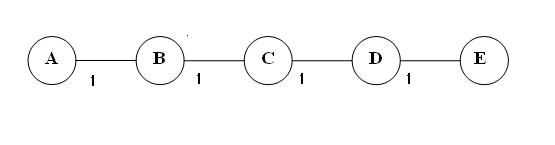
\includegraphics[width=0.95\textwidth]{./figures/VectorDistancia1}		
	\caption{\textit{Topología de red para ejemplificar la limitación del protocolo $vector$ $distancia$.}}
	\label{figuraVectorDistancia1}
\end{figure}

\begin{itemize}
\item Inicialmente A está desactivado. Cuando A se activa, B se entera de que A existe al recibir su vector distancia y actualizar su tabla indicando que A dista 1.

\item El nodo C se entera de que A existe porque B le indica que tiene un enlace hacia A de coste 1. Entonces C actualiza su tabla registrando una trayectoria hacia A de coste 2.

\item Si el nodo A se desconecta entonces B no recibe el VD de A. Sin embargo el nodo C le dice que tiene una trayectoria hasta A de distancia 2. B no sabe que la trayectoria de C a A pasa por el mismo y por tanto cree que puede llegar a A a través de C por lo que actualiza su tabla registrando la distancia 2 + 1 = 3 hasta A.

\item En el siguiente intercambio, el nodo C comprueba que sus vecinos B y D tienen una trayectoria hasta A de distancia 3. C calcula su propia distancia hasta A en 3 + 1 = 4. En los siguientes intercambios, los nodos elevan ilimitadamente su distancia a A (cuenta a infinito).
\end{itemize}

Mientras no se interrumpa la cuenta a infinito, el algoritmo no converge. Aunque se han propuesto diversas soluciones a este problema. El protocolo RIP establece el siguiente criterio:

\begin{center}
$ \infty = 16. $
\end{center}

Es decir, cuando la cantidad de incrementos de distancia supera los 15 en un período de tiempo relativamente corto, RIP considera que se está en un loop infinito y corta las iteraciones. El protocolo OLSR utiliza un acercamiento más eficiente, como se verá en (\ref{subseccionProtocoloOLSR}).


\subsection{Protocolo OLSR}
\label{subseccionProtocoloOLSR}

El protocolo de ruteo Optimized Link State Routing (o OLSR) emplea el algoritmo de $vector$ $distancia$ pero tiene muchos menos conteos a ínfinitos que el protocolo RIP. Para mantener informados a los nodos de la red de los cambios topológicos de la misma, utiliza el mecanimo Multi-Point Relay (o MPR) para hacer flooding \footnote{Se le dice $flooding$ a la acción de enviar un paquete de actualización de métricas a $todos$ los nodos de la red. Cuando un nodo desea hacer $flooding$ primero le envía el paquete deseado a todos sus nodos vecinos. Luego, estos retransmiten el mensaje hasta que éste llegue a todos los nodos de la red.}. A diferencia del flooding convencional, el método MPR evita que todos los nodos vecinos retransmitan los paquetes. Todos los nodos de la red seleccionan entre sus vecinos un conjunto de retransmisores  (o $multi$ $point$ $relays$) encargados de retransmitir los mensajes que envía el nodo inicial. Los demas vecinos del nodo no pueden retransmitir, lo cual reduce significativamente el tráfico generado respecto al flooding tradicional.

Hay varios criterios para elegir los MPRs de un nodo. En general, se considera que el conjunto de MPRs de un nodo debe verificar que son capaces de alcanzar a todos los vecinos situados a 2 $hops$ del nodo que los define como MPR.

EL protocolo OLSR es un protocolo muy usado pero como fue desarrollado en los inicios del 2000 no está pensado para rutear información en redes mesh. De hecho, hay multiples fuentes que demuestran que OLSR sufre de muchos conteos a infinito en redes mesh \cite{PAPERbatman} y que su performance con respecto a otros protocolos de ruteo como los que se presentarán en (\ref{subseccionProtocoloBatman}), (\ref{subseccionProtocoloBabel}) y (\ref{subseccionProtocoloSSR}) es mucho menor \cite{PAPERrealWORLDperformance}.

\subsection{Protocolo BatMan}
\label{subseccionProtocoloBatman}

Mencionar la existencia de BMX7 y diferenciarlo de batman base

\subsection{Protocolo Babel}
\label{subseccionProtocoloBabel}

\subsection{Protocolo SSR}
\label{subseccionProtocoloSSR}

\subsection{Comparaciones}
\label{subseccionComparacionesProtocolosDeRuteo}
Aca podria copi-pastear el cuadro que uso el flaco de althea para su presentacion. El problema es que en ese cuadro hay 2 protocolos que no estudie. SSR porque no lo entendi y CJS... porque no estaba en ningun paper recomendado. Hay que achicar la tabla.

Aca tambien nombrar en algun momento que se puede demotrar que hay muchas brechas de seguridad (y nombrar el paper que dijo eso) y que para llegar a tener un protocolo seguro habria que definir y estandarizar un conjunto de criterios de protocolo seguro ( y citar el paper que dijo eso). Pero que no se le va a dar mucha importancia en este trabajo porque para redes que no sean militares o de informacion fiscal no hace falta (citar al paper que dijo eso ultimo tambien) y yo voy a usar redes caseras.

\section{Criptografía}

\subsection{Hashing}



